%!TEX program = xelatex
%!TEX spellcheck = en_GB
\documentclass[final]{report}
% Include all project wide packages here.
%\usepackage{fullpage}
\usepackage[a4paper,margin=2.5cm,top=2cm]{geometry}
\usepackage{polyglossia}
\setmainlanguage{english}
\usepackage{csquotes}
\usepackage{graphicx}
\usepackage{pdfpages}
\usepackage{caption}
\usepackage[list=true]{subcaption}
\usepackage{float}
\usepackage{standalone}
\usepackage{import}
\usepackage{tocloft}
\usepackage{wrapfig}
\usepackage{authblk}
\usepackage{array}
\usepackage{booktabs}
\usepackage[title,titletoc]{appendix}
\usepackage{fontspec}
\usepackage{pgfplots}
\usepackage{tikz}
\usepackage[binary-units=true]{siunitx}
\usepackage{units}
\usepackage{amsmath}
\usepackage{mathtools}
\usepackage{unicode-math}
\usepackage{rotating}
\usepackage{titlesec}
\usepackage{titletoc}
\usepackage{blindtext}
\usepackage{color}
\usepackage{enumitem}
\usepackage{tabularx}
\usepackage{titling}
\usepackage[%
siunitx,
fulldiodes,
europeanvoltages,
europeancurrents,
europeanresistors,
americaninductors,
smartlabels]{circuitikz}

\newcommand{\matlab}{{\textsc{matlab }}}

\usetikzlibrary{calc}
\usetikzlibrary{positioning}
\usetikzlibrary{automata}
\usetikzlibrary{arrows.meta}

\tikzstyle{every state}=[fill=tu-cyan,align=center,draw=black,line width=1pt,node distance=3cm,minimum width = 1.8cm]%for FSMs casper
\tikzstyle{every initial by arrow}=[initial text={Reset}]
\newcommand{\setpathasarrows}{\tikzstyle{every path}=[auto,line width=1.5pt,line cap=round,line join=round]}

\pgfplotsset{compat=newest}
\pgfplotsset{plot coordinates/math parser=false}
\usetikzlibrary{plotmarks}
\usepgfplotslibrary{patchplots}
\newlength\figureheight
\newlength\figurewidth

\tikzset{every axis/.style={xticklabel style={align=right}}}

\usepackage[
%backend=bibtex,
backend=biber,
	texencoding=utf8,
bibencoding=utf8,
style=numeric,
citestyle=numeric,
    sortlocale=en_US,
    language=auto,
    backref=true,
    abbreviate=false,
    date=edtf,
    seconds=true
]{biblatex}


\usepackage{listings}
\newcommand{\includecode}[4][c]{\lstinputlisting[caption=#2, escapechar=, style=#1,label=#4]{#3}}
\newcommand{\superscript}[1]{\ensuremath{^{\textrm{#1}}}}
\newcommand{\subscript}[1]{\ensuremath{_{\textrm{#1}}}}


\newcommand{\chapternumber}{\thechapter}
\renewcommand{\appendixname}{Appendix}
\renewcommand{\appendixtocname}{Appendices}
\renewcommand{\appendixpagename}{Appendices}


\setlist[enumerate]{labelsep=*, leftmargin=1.5pc}
\setlist[enumerate,1]{label=\arabic*., ref=\arabic*}
\setlist[enumerate,2]{label=\arabic*.,ref=\theenumi.\arabic*}
\setlist[enumerate,3]{label=\arabic*., ref=\theenumii.\arabic*}

%\setcounter{chapter}{-1} %start chapter numbers with 0

\usepackage{xr-hyper}
\usepackage[hidelinks]{hyperref} %<--------ALTIJD ALS LAATSTE
\usepackage[nameinlink,noabbrev,capitalise]{cleveref} %<------- Clever Ref moet na hyperref
\crefname{app}{Appendix}{Appendices}
%\renewcommand{\familydefault}{\sfdefault}


\setmainfont{Myriad Pro}[Ligatures={Common,TeX}]
\setmathfont{Asana Math}
\setmonofont[Scale=0.9]{Lucida Console}
\newfontfamily\headingfont{Minion Pro}[Ligatures={Common,TeX}]


%Design colors
\definecolor{accent1}{RGB}{0,100,200}
\definecolor{accent2}{RGB}{0,50,100}
\definecolor{tu-cyan}{RGB}{0,166,214}

\newcommand{\hsp}{\hspace{20pt}}
\titleformat{\chapter}[hang]{\Huge\headingfont}{\chapternumber\hsp\textcolor{accent2}{|}\hsp}{0pt}{\Huge\headingfont}

\titleformat{name=\chapter,numberless}[hang]{\Huge\headingfont}{\hsp\textcolor{accent2}{|}\hsp}{0pt}{\Huge\headingfont}

\titleformat{\section}[block]{\LARGE\headingfont}{\arabic{chapter}.\arabic{section}}{0.4em}{}
\titleformat{\subsection}[block]{\Large\headingfont}{\arabic{chapter}.\arabic{section}.\arabic{subsection}}{0.4em}{}
\titleformat{\subsubsection}[block]{\large\headingfont}{\arabic{chapter}.\arabic{section}.\arabic{subsection}.\arabic{subsubsection}}{0.4em}{}
\renewcommand{\arraystretch}{1.2}
\renewcommand{\baselinestretch}{1.25} 

\renewcommand\cfttoctitlefont{\headingfont\Huge}
\renewcommand\cftloftitlefont{\headingfont\Huge}
\renewcommand\cftlottitlefont{\headingfont\Huge}
\setcounter{lofdepth}{2}
\setcounter{lotdepth}{2}


\setlength{\parindent}{0pt}
\setlength{\parskip}{1em}


%SIuntix settings:
%default: 0V to 10V
%custom: 0 - 10V
\sisetup{range-phrase=--}
\sisetup{range-units=single}
\DeclareSIUnit\years{years}

%For code listings
\definecolor{black}{rgb}{0,0,0}
\definecolor{browntags}{rgb}{0.65,0.1,0.1}
\definecolor{bluestrings}{rgb}{0,0,1}
\definecolor{graycomments}{rgb}{0.4,0.4,0.4}
\definecolor{redkeywords}{rgb}{1,0,0}
\definecolor{bluekeywords}{rgb}{0.13,0.13,0.8}
\definecolor{greencomments}{rgb}{0,0.5,0}
\definecolor{redstrings}{rgb}{0.9,0,0}
\definecolor{purpleidentifiers}{rgb}{0.01,0,0.01}


\lstdefinestyle{csharp}{
language=[Sharp]C,
showspaces=false,
showtabs=false,
breaklines=true,
showstringspaces=false,
breakatwhitespace=true,
escapeinside={(*@}{@*)},
columns=fullflexible,
commentstyle=\color{greencomments},
keywordstyle=\color{bluekeywords}\bfseries,
stringstyle=\color{redstrings},
identifierstyle=\color{purpleidentifiers},
basicstyle=\ttfamily\small}

\lstdefinestyle{c}{
language=C,
showspaces=false,
showtabs=false,
breaklines=true,
showstringspaces=false,
breakatwhitespace=true,
escapeinside={(*@}{@*)},
columns=fullflexible,
commentstyle=\color{greencomments},
keywordstyle=\color{bluekeywords}\bfseries,
stringstyle=\color{redstrings},
identifierstyle=\color{purpleidentifiers},
}

\lstdefinestyle{matlab}{
language=Matlab,
showspaces=false,
showtabs=false,
breaklines=true,
showstringspaces=false,
breakatwhitespace=true,
escapeinside={(*@}{@*)},
columns=fullflexible,
commentstyle=\color{greencomments},
keywordstyle=\color{bluekeywords}\bfseries,
stringstyle=\color{redstrings},
identifierstyle=\color{purpleidentifiers}
}

\lstdefinestyle{vhdl}{
language=VHDL,
showspaces=false,
showtabs=false,
breaklines=true,
showstringspaces=false,
breakatwhitespace=true,
escapeinside={(*@}{@*)},
columns=fullflexible,
commentstyle=\color{greencomments},
keywordstyle=\color{bluekeywords}\bfseries,
stringstyle=\color{redstrings},
identifierstyle=\color{purpleidentifiers}
}

\lstdefinestyle{xaml}{
language=XML,
showspaces=false,
showtabs=false,
breaklines=true,
showstringspaces=false,
breakatwhitespace=true,
escapeinside={(*@}{@*)},
columns=fullflexible,
commentstyle=\color{greencomments},
keywordstyle=\color{redkeywords},
stringstyle=\color{bluestrings},
tagstyle=\color{browntags},
morestring=[b]",
  morecomment=[s]{<?}{?>},
  morekeywords={xmlns,version,typex:AsyncRecords,x:Arguments,x:Boolean,x:Byte,x:Char,x:Class,x:ClassAttributes,x:ClassModifier,x:Code,x:ConnectionId,x:Decimal,x:Double,x:FactoryMethod,x:FieldModifier,x:Int16,x:Int32,x:Int64,x:Key,x:Members,x:Name,x:Object,x:Property,x:Shared,x:Single,x:String,x:Subclass,x:SynchronousMode,x:TimeSpan,x:TypeArguments,x:Uid,x:Uri,x:XData,Grid.Column,Grid.ColumnSpan,Click,ClipToBounds,Content,DropDownOpened,FontSize,Foreground,Header,Height,HorizontalAlignment,HorizontalContentAlignment,IsCancel,IsDefault,IsEnabled,IsSelected,Margin,MinHeight,MinWidth,Padding,SnapsToDevicePixels,Target,TextWrapping,Title,VerticalAlignment,VerticalContentAlignment,Width,WindowStartupLocation,Binding,Mode,OneWay,xmlns:x}
}

\lstdefinestyle{python}{
language=Python,
showspaces=false,
showtabs=false,
breaklines=true,
showstringspaces=false,
breakatwhitespace=true,
escapeinside={(*@}{@*)},
columns=fullflexible,
commentstyle=\color{greencomments},
keywordstyle=\color{bluekeywords}\bfseries,
stringstyle=\color{redstrings},
identifierstyle=\color{purpleidentifiers},
}

%defaults
\lstset{
basicstyle=\ttfamily\scriptsize ,
extendedchars=false,
numbers=left,
numberstyle=\ttfamily\tiny,
stepnumber=1,
tabsize=4,
numbersep=5pt
}
\addbibresource{../../.library/bibliography.bib}
\begin{document}
\chapter{Dataset and Results}
\label{ch:dataset}

%From Analysis:
This section describes how the data that was gathered in the previous steps will be analysed using the proper tools. The main goal is to see whether certain toxic users are only toxic when they are viewing a certain streamer or in every channel they visit. So whether viewers match their toxicity level to the channel. Another interesting question is to see if certain channels are more toxic than others and how this affects the toxicity levels of the users. 

\section{Streamers per User}
Twitch users like to view different games. And therefore watch to different Streamers. In this dataset there are a lot of users that only watch streams of one streamer. But there are also a lot that wath streams of other streamers. In Figure \ref{fig:streamPerUser} the streamers per users are plot on a logaritmic scale. In the original dataset there were users that watched to even more streamers, but those were bots. The user on top of this list was present in all chat rooms, because this was a bot from twitch itself, to place notifications in the chat.\\
If we had more data aboutthe toxicity of users we could see if users that are toxic in one chat are only toxic by that streamer, or by multiple. 

\begin{figure}[h]
	\centering
	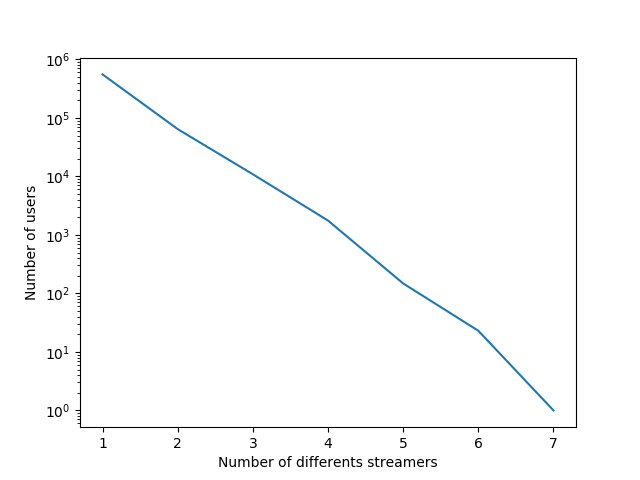
\includegraphics[width=0.7\textwidth]{StreamersPerUser.png}
	\caption{Streamers per User}
	\label{fig:streamPerUser}
\end{figure}

\noindent
\begin{minipage}{.5\textwidth}
  
\section{Wordcount}
One of the things we can get from our dataset is the number of times a certain word is used.
Certain words are expected to occur a lot. These are words used in the english language a lot. A lot of articles, like "the", are seen. Also team names are found on top of this list. To be able to analyze these results better, team names, articles and a few other words are left out. The first 25 words of this filtered list is shown in Table \ref{wordcounttabel}.\\
The one on top, "vac", is said the most. It most likely is said when a user thinks someone is cheating. This conclusion is made because VAC is the name off the anti-cheat system of Valve (Valve Anti-Cheat System). Valve is the creator of Steam, a platform for games. The word "VAC" can be seen as toxic, because it is an accusation towards the streamer, or the other players in the game."VAC" is said a lot when a player in the game does something that is almost impossible, so it could also be jealousy from the user.\\
In the dataset we see that Twitch users like to say where they are from. That's why we see "na", "eu" and "usa" high in this list. "na" most likely stands for North America and "eu" is the European Union. The words are not toxic by themselves, but there could start a discussion by the users about what continent or country is better and with that toxic comments are possible.\\
"fuck" is high in this list, as expected. But luckaly the words "good" and "nice" occur more. Unfortunately "good" and "nice" could also be used in a toxic way. When they are used in a sarcastic way, the sentence will be toxic. 

\end{minipage}% This must go next to `\end{minipage}`
\begin{minipage}{.5\textwidth}
\centering
\captionof{table}{Number of times words are used.}
\label{wordcounttabel}
\begin{tabular}{|l|l|}
\hline
Word    & Wordcount \\ \hline
vac     & 134034    \\ \hline
lol     & 122647    \\ \hline
na      & 86260     \\ \hline
rip     & 46703     \\ \hline
god     & 40136     \\ \hline
nip     & 39178     \\ \hline
ez      & 37953     \\ \hline
bot     & 36822     \\ \hline
lg      & 31513     \\ \hline
drop    & 30235     \\ \hline
sourpls & 28612     \\ \hline
vp      & 27679     \\ \hline
eu      & 25986     \\ \hline
game    & 22379     \\ \hline
rekt    & 22321     \\ \hline
usa     & 22265     \\ \hline
nt      & 20692     \\ \hline
cobble  & 18345     \\ \hline
nice    & 18161     \\ \hline
good    & 17439     \\ \hline
fuck    & 17424     \\ \hline
why     & 17364     \\ \hline
faze    & 16938     \\ \hline
lmao    & 16266     \\ \hline
\end{tabular}

\end{minipage}

\section{Deleted messages}

Twitch also has it's own filtering, before it appears in the chats. Some of the messages send are therefore deleted by Twitch. The messages that are deleted are however avaiable in the rechat log. However, the message itself is removed by the deleted flag is set to true. This way we can still analyse some of the data.\\
There are some interesting facts to detect about the deleted messages:
\begin{itemize}
	\item Ratio of deleted messages per user
	\item Ratio of deleted messages per stream
\end{itemize}


\subsection{Deleted messages per user}
We wanted to see if a users behaves the same way in different video's. If this is the case, one could conclude that the toxicity is due the user and not the streamer. If the looks random, one could conclude that the streamer has more influence to the toxicity of the users.

However, this is very hard to visualize and generalize for different users/streamers of the entire dataset.
Because of this, we took a one streamer (AmazHS) and picked some videos and compared them.

\begin{verbatim}
[('datguyzed', 0.416), ('everdreen', 0.181)]
[('awildchocobo', 0.727), ('rommikoira', 0.571), ('maedalislie', 0.428)]
[('leckotut', 0.166)]
[('koran_mekka', 0.5)]
[('sokkimhong', 0.833), ('awesomememesspammedquick', 0.545), ('moonmoonderp', 0.5)]
[('jroblul', 0.636), ('silentdropx', 0.615), ('paskajaakko420', 0.4375)]
[('yoshinami', 0.454)]
[('generalkkona', 0.416), ('quietguy89', 0.207), ('srbombarder', 0.190)]
[('leckotut', 0.666), ('matt_friday', 0.12)]
[('comi_', 0.428)]
[('everdreen', 0.2)]
[('m9za', 0.714), ('sahrgeand', 0.692), ('veelyo', 0.111), ('drsmoke100', 0.091)]
[('leecolas', 0.307), ('gunnervine', 0.176), ('nielsnice', 0.133), ('lockiez', 0.066)]
[('meezy_money', 0.384)]
\end{verbatim}

As can be seen, there isn't a pattern visible. So it looks that the users are randomly being toxic.\\
However, it's very likely that we have not enough data to get such results. It's possible that we don't have the same users watching, and that the toxic users only appear in one video.

\subsection{Deleted messages per stream}
Before we calculate the ratio, we want to filter the data some more. We exclude all the users in a single chatlog that have posted less than 10 messages. So only users that posted more than 10 messages are considered 'real' users, that tend to watch the stream. 
We sum all ratio's of the users in a stream and calculate the average ratio. Then we plot the ratio against the amount of users with that ratio in figure \ref{fig:deletedPerStream}. The amount of users are normalized, so we can compare different sizes of streamers.
In figure \ref{fig:deletedPerStream} we took the three largest streamers in our dataset. Note that the largest streamer (MLG) has around 35000 users that had a message deleted. The second (eleaguetv) has around 10000 users and the third (dreamhackcs) only around 700.

\begin{figure}[h]
	\centering
	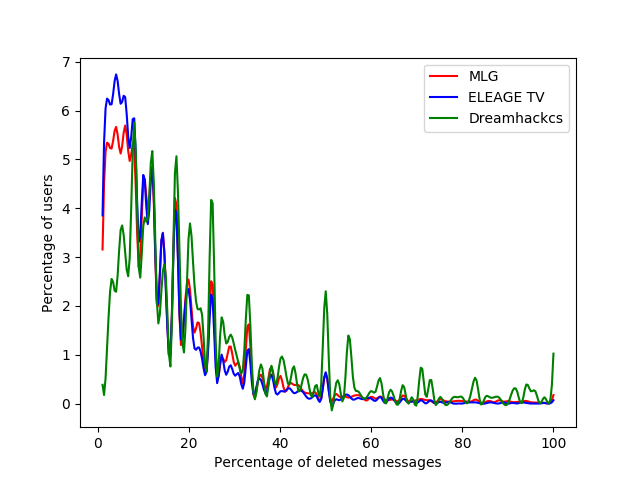
\includegraphics[width=0.7\textwidth]{DeletedPerStreamer.png}
	\caption{Ratio of deleted messages in a stream}
	\label{fig:deletedPerStream}
\end{figure}

As can be seen, the MLG stream has the most amount of low ratio users, and the amount decreases as the ratio increases. However, in the dreamhackcs data we see that the lowest ratio doesn't have the highest amount of users. The line increases in the beginning and the most users with deleted message have a ratio around 10-20$\%$. After this peak all streams show a similar pattern toward a higher ratio.
However, and the end we see a jump at a ratio of 1. These are the users that got all of their messages deleted (10+ messages).\\

We can also compare the total amount of messages in a channel, and compare that to the average ratio in the entire channel. We see that the bigger the streamer, the higher the ratio. However the ratio's are very close to eachother, and there are a lot of other factors (game, time of day, etc) involved to say that the bigger the channel, the more toxic it becomes. In the appendix is the full list for all streamers.

\begin{table}[]
\centering
\caption{Ratio and message data per streamer}
\label{my-label}
\begin{tabular}{l|lll}
Streamer 		 & Deleted messaged & Total messages 	& Ratio 	\\
mlg              & 301688 			& 2628092 			& 0.1148   	\\
eleaguetv        & 60761  			& 779918  			& 0.0779   	\\
dreamhackcs      & 8190   			& 112943  			& 0.0725	\\
\end{tabular}
\end{table}



\end{document}